\documentclass[11pt,a4paper]{article}

\usepackage[utf8]{inputenc}
\usepackage[T1]{fontenc}
\usepackage[spanish,english]{babel}
\usepackage{lmodern}
\usepackage{microtype}
\usepackage[margin=2.5cm]{geometry}
\usepackage{booktabs}
\usepackage{array}
\usepackage{graphicx}
\usepackage{caption}
\usepackage{subcaption}
\usepackage{amsmath}
\usepackage{hyperref}
\usepackage{xcolor}
\usepackage{natbib}
\usepackage{authblk}
\usepackage{siunitx}
\usepackage{eurosym}

\hypersetup{
  colorlinks=true,
  linkcolor=blue!50!black,
  citecolor=blue!50!black,
  urlcolor=blue!50!black,
}

\title{\textbf{Capacity Market Design and Renewable Investment in Spain:}\\
       \large A forensic audit of the \emph{derating factors} of the 2026
       capacity mechanism (SA.112483 / RD 932/2024) using hourly ELCC data
       (2019--2024)}
\author{Carlo Vilches}
\affil{Universitat de Barcelona\\
       \texttt{cvilchce15@alumnes.ub.edu}}
\date{\today}

\begin{document}
\selectlanguage{english}
\maketitle

\begin{abstract}
\noindent
On 29 May 2026 the European Commission approved, under Article 107(3)(c) TFEU,
a \EUR{9} billion, ten-year capacity mechanism (CM) for Spain (case SA.112483),
in which the system operator remunerates every megawatt \emph{available during a
scarcity event} through competitive auctions \citep{ec2026sa112483}. The
parameter that translates nominal capacity into accreditable megawatts ---the
\emph{derating factor}--- ceases to be an academic abstraction and becomes the
variable that allocates \EUR{900} million per year across technologies. This paper
audits that parameter. We quantify the \emph{Effective Load Carrying Capability}
(ELCC) of six technologies of the Spanish peninsular system using hourly ENTSO-E
data (BZN\textbar ES, 2019--2024) and show that three seemingly technical
calibration choices create first-order incentive distortions and regulatory
arbitrage risks: (i) treating hydro as an aggregate ($\text{ELCC}=0.22$)
under-remunerates reservoir hydro ($0.73$) and pumped storage ($0.64$) by a factor
of $\sim$3$\times$ and over-remunerates run-of-river ($0.14$), generating
\emph{adverse selection} in the auction and destroying the investment signal for
storage; (ii) importing northern-European solar \emph{derating factors}
($0.01$--$0.03$) ignores the Spanish bimodal profile
($\text{ELCC}_{\text{solar}}=0.13$, summer cooling peaks) and penalises solar
\emph{missing money} by $\sim$80\%; (iii) calibrating gas on the raw history
imports a regulatory artifact ---the Iberian Exception (2022--2023) inflated CCGT
ELCC by $+0.072$ ($+19\%$)--- buying fictitious physical security. Finally,
cross-checking with the MIBEL Congestion Monitor (Jaccard $\leq 0.10$ between price
stress and the top of net demand) confirms that the CM must penalise non-delivery
on \emph{physical} adequacy stress, not on \emph{day-ahead} financial volatility.
The frame is not ``we have computed Spain's ELCC'': it is \emph{how to calibrate
the 2026 CM without distorting investment in storage or paying inflated premiums to
gas}.
\end{abstract}

\textbf{Keywords:} Capacity mechanism, SA.112483, RD 932/2024, ELCC,
\emph{derating factors}, adverse selection, \emph{missing money}, regulatory
arbitrage, ENTSO-E, MIBEL.

% ============================================================================
\section{Introduction}
% ============================================================================

\subsection{Motivation: a \EUR{9} billion mechanism that pays per firm megawatt}

The Spanish capacity mechanism has moved from a regulatory proposal to a budgeted
transfer. Royal Decree 932/2024 \citep{rd2024cm} established its internal
architecture, and on 29 May 2026 the European Commission authorised it under State
aid rules: a \emph{market-wide} mechanism of \EUR{9} billion over ten years
(\textasciitilde\EUR{900} million/year) in which the transmission system operator
(TSO) ``remunerates all the capacity needed to meet the reliability standard'' and
beneficiaries ``compete based on the amount of aid requested per MW of capacity
available during a scarcity event'' \citep{ec2026sa112483}. Approval rests on
Article 107(3)(c) TFEU, the CEEAG 2022 Guidelines \citep{ceeag2022}, and declares
alignment with most of the best practices for capacity mechanisms of the
\emph{Clean Industrial State Aid Framework} (CISAF) \citep{cisaf2025}.

The operative phrase ---``per MW available during a scarcity event''--- is exactly
the definition of ELCC. The \emph{derating factor} is the fraction of nominal
capacity each technology can accredit as firm before the auction; multiplied by
installed capacity and by the clearing price, it sets each project's capacity
revenue. Mis-calibrating it is not an academic rounding error: it mis-allocates
\EUR{900} million a year and emits a biased investment signal over a ten-year
horizon.

\subsection{From descriptive calculation to incentive audit}

The ELCC literature is usually framed as a descriptive exercise: measuring each
technology's adequacy contribution. This paper deliberately takes a different
stance. We treat each calibration choice of the 2026 CM as an auditable hypothesis
and ask: \emph{what incentive distortion or regulatory-arbitrage risk does it
introduce?} A well-designed CM, in the Commission's own words, must not (i) raise
prices for consumers, (ii) grant undue advantages to specific operators, nor (iii)
hinder cross-border flows \citep{ec2026sa112483}. We show that three common
calibration shortcuts directly violate criterion (ii) ---undue advantages--- via
mis-specified \emph{derating factors}.

\subsection{Research question}

What are the empirically justified \emph{derating factors} for the relevant
technologies (nuclear, wind, solar, reservoir hydro, run-of-river, pumped storage,
gas) in the peninsular system 2019--2024, and what auction distortions does the
2026 CM generate if calibrated with the usual shortcuts (aggregated hydro, imported
benchmarks, uncleaned history, price-based activation)? To what extent are the
findings robust to the temporal granularity of the data and to the internal split
of hydro capacity?

\subsection{Contribution}

\begin{enumerate}
\item \textbf{ELCC from real hourly data} (ENTSO-E 16.1.B\&C, BZN\textbar ES,
      2019--2024) instead of token-free daily generation (REData). For
      dispatchable technologies with a concentrated temporal profile, the hourly
      peak capacity factor differs materially from the daily one.
\item \textbf{Disaggregation of hydro} into its three sub-technologies (reservoir,
      run-of-river, pumped storage). The traditional aggregate conceals an adequacy
      heterogeneity of factor 5$\times$, validated through a sensitivity analysis
      over five capacity-split scenarios.
\item \textbf{Quantification of the regulatory bias} of the Iberian Exception
      (2022--2023) on gas ELCC ($+0.072$).
\item \textbf{Translation into design risks}: we map each statistical finding onto
      a named auction risk of the 2026 CM (adverse selection, \emph{missing
      money}, regulatory artifact, price-based activation), with the corresponding
      calibration recommendation.
\end{enumerate}

% ============================================================================
\section{Literature}
% ============================================================================

\citet{garver1966} introduced ELCC as a metric of equivalence between capacity
additions and demand reductions: a unit with ELCC=1.0 is equivalent, from an
adequacy standpoint, to a permanent 1\,MW reduction of peak demand. It is this
equivalence that the 2026 CM monetises by paying ``per MW available in scarcity''
\citep{ec2026sa112483}.

\citet{millswiser2013} and \citet{madaeni2013} formalise the various approaches to
computing ELCC under growing renewable penetration, identifying the
``saturation'' or dilution effect of marginal ELCC as the installed capacity of
technologies with correlated profiles increases.

The debate over the need for capacity mechanisms proper ---versus an
\emph{energy-only} design--- is consolidated in \citet{joskow2008} and
\citet{cramton2013}. \citet{batlleperezarriaga2008} discuss specific design
criteria for liberalised markets, prefiguring elements of RD 932/2024. The current
European framework ---Regulation (EU) 2019/943 \citep{euelectricityreg}, CEEAG 2022
\citep{ceeag2022} and CISAF \citep{cisaf2025}--- requires the CM to be
proportionate and non-discriminatory, which in practice hinges on the quality of
the \emph{derating factors}.

The European benchmarks published by \citet{nationalgrideso2024},
\citet{eirgrid2023} and \citet{pse2023} serve as comparative references, but their
transferability to the Spanish case is limited by differences in climatic profile
and technology mix ---a point that Axis~2 (Section~\ref{sec:eje2}) turns into a
quantified risk.

% ============================================================================
\section{Data}
% ============================================================================

\subsection{Generation: ENTSO-E BZN\textbar ES (hourly, 2019--2024)}

We download the 72 monthly files of the ``Actual Generation per Production Type''
dataset (16.1.B\&C, area code 10YES-REE---0). The official unit is the
interval-average MW \citep{entsoe2023}: for PT60M (2019-01 to 2022-05) and PT15M
(from 2022-06) the conversion to MWh per hour is either direct (PT60M) or requires
a moving average (PT15M $\rightarrow$ PT60M with the mean). Coverage is 99.94\%
(5 hours missing on 2019-12-24 02--06h UTC, a source gap).

The dataset includes 21 \emph{Production Types}; this work uses seven: nuclear
(B14), solar (B16), wind onshore+offshore (B19+B18), reservoir hydro (B12),
run-of-river (B11), pumped storage (B10) and \emph{Fossil Gas} (B04).

\subsection{Installed capacity: REData (REE)}

REData publishes monthly installed capacity by technology (\texttt{api.ree.es}, no
token). It is forward-filled to hourly resolution to align with ENTSO-E
generation. The aggregate ``Hydro'' capacity (\textasciitilde17 GW) is not broken
down into reservoir, run-of-river and pumped storage; the 35/45/20\% split is used
(\emph{Section 6.4}), validated by sensitivity.

\subsection{Geographic coverage}

ENTSO-E BZN\textbar ES corresponds to the peninsular system plus the Balearic
Islands; it excludes the Canary Islands. REData generation-by-structure includes
the Canaries. The annual difference in wind is roughly $-3\%$ (consistent with
\textasciitilde2 TWh/year of Canary wind), absorbed as a documented caveat. The
peninsular coverage is the relevant one: SA.112483 opens the mechanism to projects
``located in Spain'' within the interconnected peninsular system
\citep{ec2026sa112483}.

\subsection{Systemic stress: MIBEL Congestion Monitor}

For Axis~4 (Section~\ref{sec:eje4}) we reuse the 52\,530 hours classified by
\citet{vilches2024mibel}, of which 1\,044 are Orange or Red alerts (1.99\% of the
total).

% ============================================================================
\section{Methodology}
% ============================================================================

\subsection{\emph{Naive} ELCC}

\begin{equation}
\text{ELCC}(\text{tech}, N) = \frac{\overline{\text{gen}}_{\text{tech}}(\mathcal{T}_N)}{\bar{C}_{\text{tech}}(\mathcal{T}_N)\cdot \Delta t}
\label{eq:elcc}
\end{equation}

where $\mathcal{T}_N$ are the $N$ records (days in \texttt{daily}; hours in
\texttt{hourly}) with the highest net demand in the period, $\bar{C}$ is the mean
installed capacity over those records, and $\Delta t$ is the interval duration
(24h or 1h). Net demand:
$D^{net} = \sum_i \text{gen}_i - \text{gen}_{\text{wind}} - \text{gen}_{\text{solar}}$.

For \texttt{daily} we use $N=100$ (top-100 days, matching the convention of
\citet{entsoe2023}); for \texttt{hourly}, $N=2\,400$ (top-2\,400 hours, the same
temporal volume).

\subsection{Marginal ELCC}

Following \citet{millswiser2013} it is approximated by a finite difference:
\begin{equation}
\text{marginal\_ELCC}(\text{tech}) = \frac{\text{ELCC}(C+\Delta C) - \text{ELCC}(C)}{\Delta C}
\label{eq:marginal}
\end{equation}

with $\Delta C = 1$\,GW. The operational assumption is that generation in peak
hours does not increase when capacity is added (dispatch saturation); this provides
an upper bound on the dilution from additional capacity. By construction, all
marginals are negative.

\subsection{Market regimes}

The period is segmented into three regimes:
\begin{itemize}
\item \emph{Pre-crisis}: 2019-01-01 to 2021-12-31.
\item \emph{Iberian Exception}: 2022-01-01 to 2023-12-31 (gas adjustment mechanism,
      RDL 10/2022).
\item \emph{Post-exception}: 2024-01-01 onwards (return to the ordinary regime with
      high renewable penetration).
\end{itemize}

The \emph{regulatory bias} of a technology is defined as the difference between its
ELCC over the full period and its ELCC excluding the Iberian Exception.
Operationally, it is the fictitious firmness premium the 2026 CM would ``buy'' if
calibrated on the raw history.

% ============================================================================
\section{Results}
% ============================================================================

\subsection{ELCC by technology: \emph{daily} vs \emph{hourly}}

Table~\ref{tab:elcc-comparison} summarises the ELCC obtained with both
granularities, restricted to the period without the Iberian Exception. For nuclear,
solar and wind the values converge ($|\Delta| < 0.01$), confirming methodological
robustness. The significant differences appear in hydro and gas ---precisely the
technologies on which the 2026 CM calibration risk falls.

\begin{table}[ht]
\centering
\caption{ELCC by technology, \emph{daily} (REData) vs \emph{hourly} (ENTSO-E),
         without the Iberian Exception, $N$ equivalent to 100 days.}
\label{tab:elcc-comparison}
\begin{tabular}{lccc}
\toprule
Technology & ELCC \emph{daily} & ELCC \emph{hourly} & $\Delta$ \\
\midrule
Nuclear                       & 0.927 & 0.919 & $-0.008$ \\
Solar (PV+T)                  & 0.126 & 0.126 & $+0.000$ \\
Wind                          & 0.152 & 0.145 & $-0.007$ \\
Total hydro                   & 0.222 & 0.334 & $+0.112$ \\
\quad Reservoir hydro         & ---   & 0.728 & new      \\
\quad Run-of-river hydro      & ---   & 0.139 & new      \\
\quad Pumped hydro            & ---   & 0.642 & new      \\
CCGT (\emph{daily}) / Fossil Gas (\emph{hourly}) & 0.372 & 0.457 & $+0.085$ \\
\bottomrule
\end{tabular}
\end{table}

\subsection{Finding: disaggregated hydro}

Table~\ref{tab:elcc-comparison} contains the paper's main finding. The
``Hydro = 0.22'' aggregate of the daily approach is an opaque average of three very
different technologies:

\begin{itemize}
\item \textbf{Reservoir} (\textasciitilde 35\% capacity): ELCC = 0.728. Almost as
      firm as nuclear.
\item \textbf{Pumped storage} (\textasciitilde 20\% capacity): ELCC = 0.642.
      Dispatchable, optimised for peak hours.
\item \textbf{Run-of-river} (\textasciitilde 45\% capacity): ELCC = 0.139. Low, as
      expected (non-dispatchable).
\end{itemize}

The economic interpretation of this dispersion ---adverse selection in the
auction--- is developed in Axis~1 (Section~\ref{sec:eje1}).
Figure~\ref{fig:heatmap-hourly} shows ELCC by threshold $N$ for all hourly
technologies.

\begin{figure}[ht]
\centering
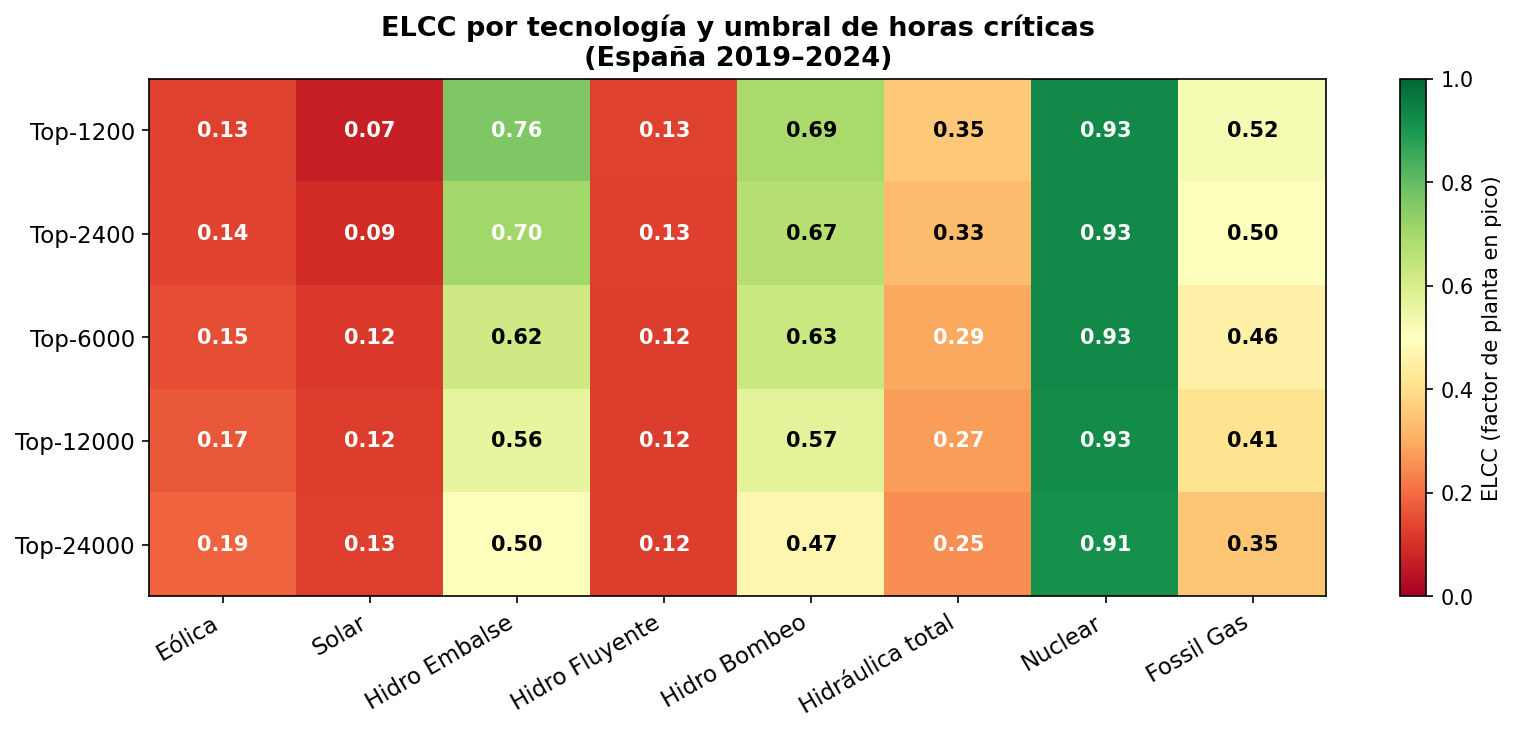
\includegraphics[width=0.95\linewidth]{../figures/block_b_1_elcc_heatmap_hourly.png}
\caption{Hourly ELCC by technology and threshold $N$. The ``Reservoir hydro''
         column is virtually flat around 0.5--0.75 across the various $N$,
         indicating high structural firmness.}
\label{fig:heatmap-hourly}
\end{figure}

\subsection{Regulatory bias: the Iberian Exception}

Table~\ref{tab:excepcion} compares ELCC with and without the Iberian Exception.
For strict CCGT (\emph{daily}, REData) the bias is $+0.072$ (+19\% relative to
0.372). For total Fossil Gas (\emph{hourly}, ENTSO-E, includes gas cogeneration)
the bias is smaller, $+0.041$, because the intervention mainly affected the
merit-order CCGT and not the non-intervened industrial cogeneration. The
calibration implication is developed in Axis~3 (Section~\ref{sec:eje3}).

\begin{table}[ht]
\centering
\caption{Regulatory bias by technology (bias $=$ ELCC$_{\text{2019-24}} -$
         ELCC$_{\text{without Iberian Exception}}$).}
\label{tab:excepcion}
\begin{tabular}{lcc}
\toprule
Technology & Bias \emph{daily} (REData) & Bias \emph{hourly} (ENTSO-E) \\
\midrule
Nuclear            & $+0.003$ & $+0.011$ \\
Wind               & $-0.024$ & $-0.009$ \\
Solar              & $+0.014$ & $-0.034$ \\
Total hydro        & $-0.025$ & $-0.005$ \\
\quad Reservoir    & ---      & $-0.024$ \\
\quad Run-of-river & ---      & $-0.010$ \\
\quad Pumped       & ---      & $+0.027$ \\
CCGT / Fossil Gas  & $\mathbf{+0.072}$ & $\mathbf{+0.041}$ \\
\bottomrule
\end{tabular}
\end{table}

\subsection{Marginal ELCC}

Table~\ref{tab:marginal} reports the marginals for $\Delta C = 1$\,GW in
\emph{hourly}. All are negative (saturation). The most pronounced correspond to
technologies with the smallest base installed capacity (pumped storage
\textasciitilde 3.4\,GW, reservoir \textasciitilde 6\,GW, nuclear
\textasciitilde 7\,GW), where an additional GW represents a proportionally large
expansion.

\begin{table}[ht]
\centering
\caption{Marginal ELCC, $\Delta C = 1$\,GW, \emph{hourly}, without the Iberian
         Exception.}
\label{tab:marginal}
\begin{tabular}{lcccc}
\toprule
Technology & Base ELCC & ELCC $+1$\,GW & Marginal & Base cap. (GW) \\
\midrule
Wind              & 0.145 & 0.140 & $-0.0053$ & 28.3 \\
Solar             & 0.126 & 0.118 & $-0.0082$ & 18.4 \\
Run-of-river      & 0.139 & 0.123 & $-0.0160$ & 7.7 \\
Pumped storage    & 0.642 & 0.497 & $\mathbf{-0.1453}$ & 3.4 \\
Reservoir         & 0.728 & 0.624 & $\mathbf{-0.1042}$ & 6.0 \\
Nuclear           & 0.919 & 0.806 & $-0.1132$ & 7.1 \\
Fossil Gas        & 0.457 & 0.441 & $-0.0161$ & 27.4 \\
\bottomrule
\end{tabular}
\end{table}

\subsection{Sensitivity to HYDRO\_CAP\_RATIOS}
\label{sec:sensitivity}

REData's aggregate hydro capacity (\textasciitilde17\,GW) is split into three
sub-technologies with approximate ratios (35/45/20\%) based on public REE
statistics. Table~\ref{tab:sensitivity} shows ELCC under five alternative scenarios
with the aggregate capacity held fixed.

\begin{table}[ht]
\centering
\caption{Sensitivity of sub-hydro ELCC to HYDRO\_CAP\_RATIOS
         (top-2\,400 hours, without the Iberian Exception).}
\label{tab:sensitivity}
\begin{tabular}{lcccc}
\toprule
Scenario & Reservoir / RoR / Pumped & Reservoir & RoR & Pumped \\
\midrule
Base                  & 35 / 45 / 20 & \textbf{0.728} & \textbf{0.139} & \textbf{0.642} \\
Conservative-reservoir & 30 / 50 / 20 & 0.849 & 0.125 & 0.642 \\
Generous-reservoir     & 40 / 40 / 20 & 0.637 & 0.156 & 0.642 \\
Conservative-pumped    & 35 / 50 / 15 & 0.728 & 0.125 & 0.856 \\
Generous-pumped        & 35 / 40 / 25 & 0.728 & 0.156 & 0.514 \\
\midrule
\multicolumn{2}{l}{\textbf{Observed range}} & \textbf{[0.64, 0.85]} & \textbf{[0.13, 0.16]} & \textbf{[0.51, 0.86]} \\
\bottomrule
\end{tabular}
\end{table}

\textbf{Robustness of the finding}: in the most adverse scenario for reservoir
(\emph{Generous-reservoir}, 40\% cap), ELCC remains 0.637 $> 0.60$. In the worst
case for pumped storage (\emph{Generous-pumped}, 25\% cap), ELCC falls to 0.514,
still clearly firm. The qualitative conclusion ``reservoir and pumped storage are
firm technologies'' holds across all five scenarios ---the adverse-selection risk
of Axis~1 does not depend on the exact split.

\subsection{Comparison with European benchmarks}

Table~\ref{tab:benchmarks} compares Spain with the UK, Ireland and Poland. The
peninsular solar ELCC ($\sim$0.13 \emph{hourly}) exceeds the UK and Irish values by
4--13$\times$. The reason is Spain's bimodal demand profile: critical hours are not
only winter-nocturnal but also summer-diurnal (cooling under high irradiance).
Figure~\ref{fig:hourly-profile} quantifies this bimodality, the basis of Axis~2
(Section~\ref{sec:eje2}).

\begin{table}[ht]
\centering
\caption{Spain ELCC (\emph{hourly}, without the Iberian Exception) vs published
         European benchmarks.}
\label{tab:benchmarks}
\begin{tabular}{lcccc}
\toprule
Country / System & Wind & Solar & Nuclear & Hydro \\
\midrule
\textbf{Spain (this work)} & \textbf{0.15} & \textbf{0.13} & \textbf{0.92} & \textbf{0.33}$^\dagger$ \\
UK \citep{nationalgrideso2024} & 0.08 & 0.03 & 0.92 & 0.15 \\
Ireland \citep{eirgrid2023}    & 0.10 & 0.01 & ---   & 0.20 \\
Poland \citep{pse2023}         & 0.08 & 0.02 & ---   & 0.10 \\
\bottomrule
\multicolumn{5}{l}{\small$^\dagger$ Total hydro (Reservoir 0.73, RoR 0.14, Pumped 0.64).}
\end{tabular}
\end{table}

\begin{figure}[ht]
\centering
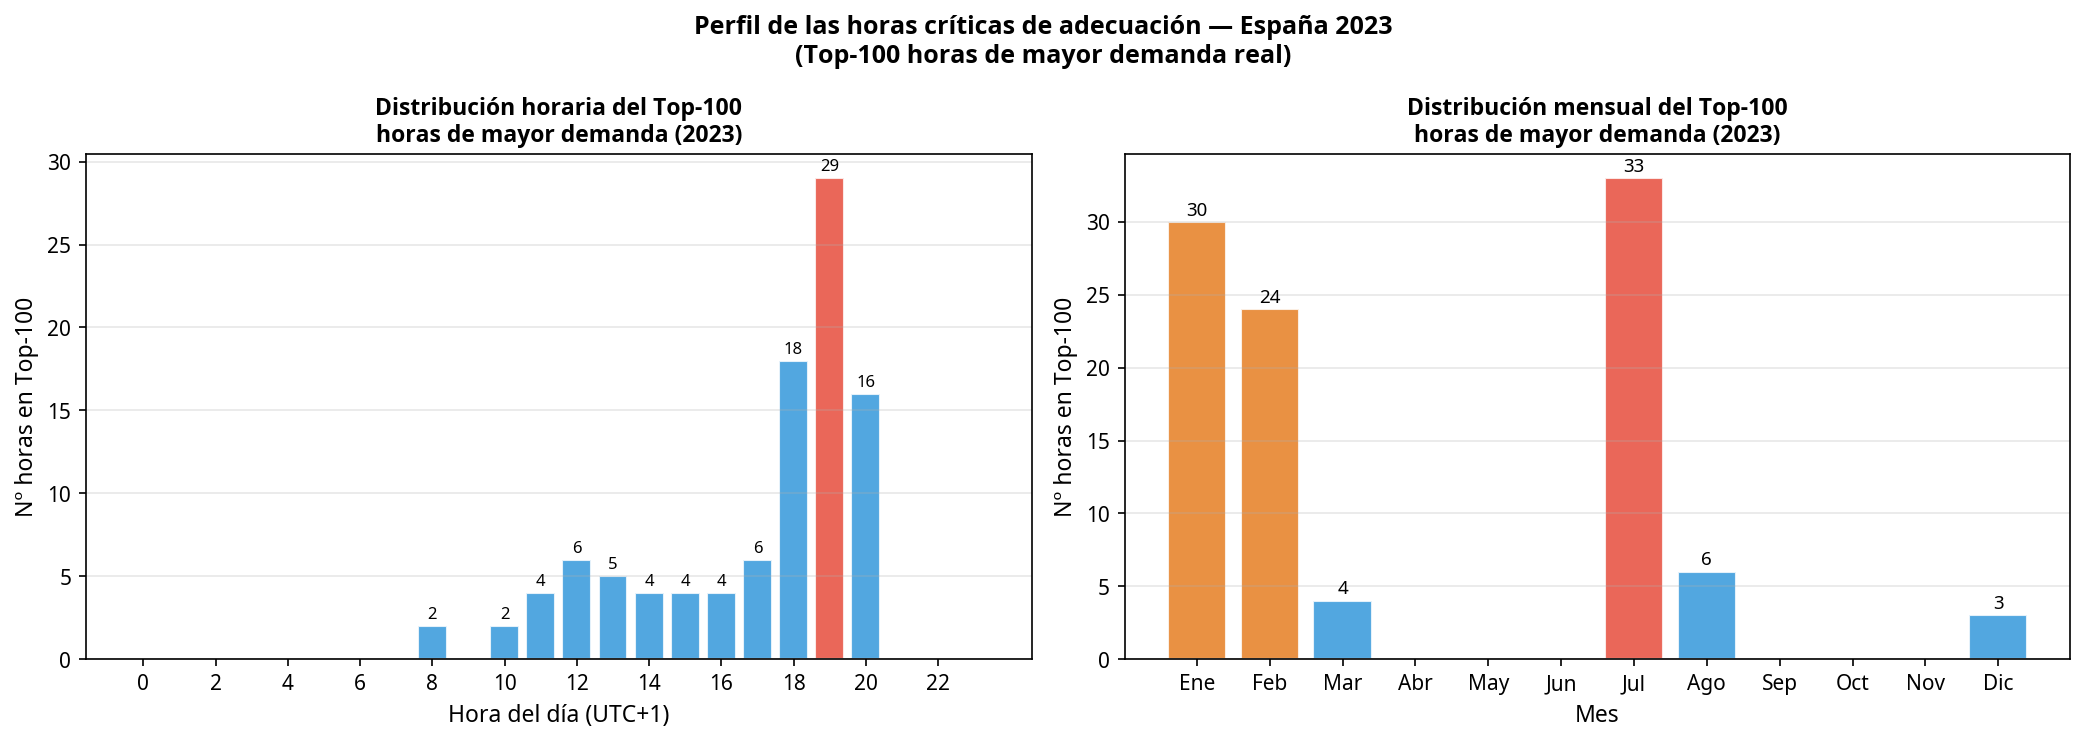
\includegraphics[width=0.9\linewidth]{../figures/block_b_6_hourly_profile_top100.png}
\caption{Hourly and monthly profile of the top-100 highest-demand hours (Spain
         2023). Double peak: winter (18--20h, Jan/Dec) and summer (12--17h,
         Jul/Aug). \textasciitilde 50\% of the critical hours have sun available.}
\label{fig:hourly-profile}
\end{figure}

\subsection{Systemic stress vs adequacy: cross-check with MIBEL}

The 1\,044 O/R hours classified by the MIBEL Congestion Monitor
\citep{vilches2024mibel} overlap with the top-$N$ highest-net-demand hours only
marginally: a Jaccard index between 0.05 (top-50) and 0.10 (top-1\,000). This
confirms that the stress detected by MIBEL ---structural tension on the ES-FR
interconnector and extreme prices--- is economic in nature, not physical adequacy.
Figure~\ref{fig:overlap} visualises this decoupling, the core of Axis~4
(Section~\ref{sec:eje4}).

\begin{figure}[ht]
\centering
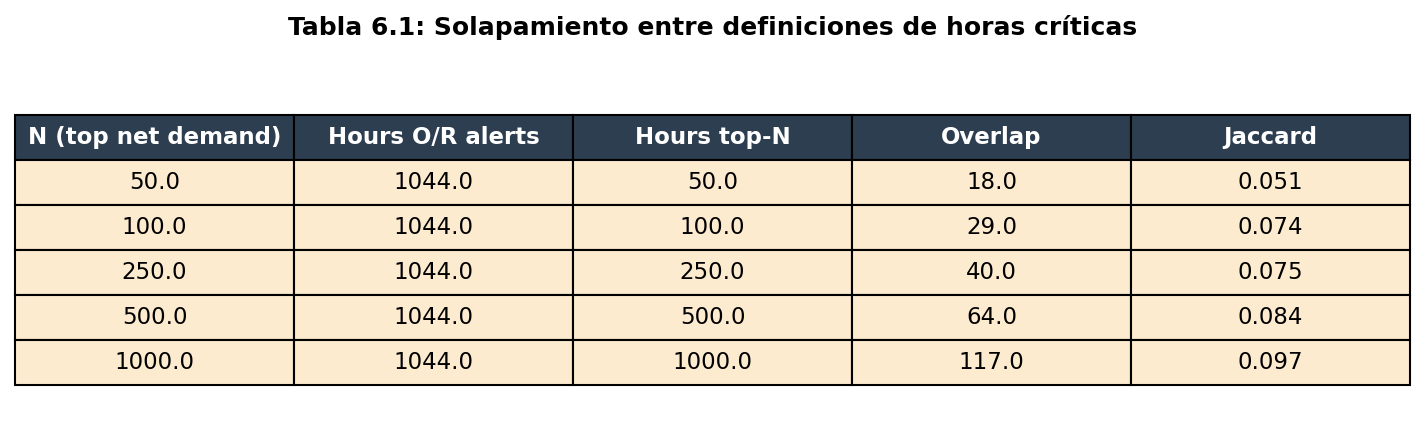
\includegraphics[width=0.85\linewidth]{../figures/block_a_2_overlap_table.png}
\caption{Overlap between MIBEL O/R alerts and the top-$N$ highest-net-demand hours.
         Jaccard $\leq$ 0.10 at every threshold: economic stress is not a proxy for
         physical insufficiency.}
\label{fig:overlap}
\end{figure}

% ============================================================================
\section{Design audit: four calibration risks of the 2026 CM}
% ============================================================================

This section translates the results of Section~5 into design risks for the
mechanism approved in SA.112483. Each axis follows the same structure: the
\emph{link} to the auction mechanics, the \emph{forensic argument} on the
distortion introduced by shortcut calibration, and the \emph{recommendation} for
correct calibration.

\subsection{Axis 1 --- Aggregated hydro: adverse selection and under-remuneration
of storage}
\label{sec:eje1}

\textbf{Link.} The auction awards a price per firm MW to each plant. The
\emph{derating factor} sets how many firm MW each unit accredits per MW installed.

\textbf{Forensic argument.} If the regulator indexes the \emph{derating factors} on
``total hydro'' ($\text{ELCC}=0.22$), the mechanism is born economically broken. It
would be \emph{under-remunerating} reservoir ($0.73$) and pumped storage ($0.64$)
by a factor close to 3$\times$, and \emph{over-remunerating} run-of-river ($0.14$)
by almost double. The result is a classic \emph{adverse-selection} problem:
run-of-river ---which, depending on instantaneous flow, cannot guarantee power in
an hour of physical stress--- receives a firmness premium it does not deserve,
while reservoir and pumped storage ---the hydro storage that does deliver power in
scarcity--- are underpaid. The long-term investment signal for storage, which
SA.112483 states it wants to foster to reach the national flexibility target
\citep{ec2026sa112483}, would be destroyed in the very first auction parameter. The
sensitivity of Section~\ref{sec:sensitivity} confirms that reservoir stays firm
($\in[0.64,0.85]$) and pumped storage too ($\in[0.51,0.86]$) across the five
scenarios: the risk is not an artifact of the assumed capacity split.

\textbf{Recommendation.} Disaggregate hydro into differentiated auctions or, at a
minimum, calibrate \emph{derating factors} specific to each production-unit code
(ESIOS), with values around $0.73$ (reservoir), $0.64$ (pumped) and $0.14$
(run-of-river). This is the only way to mitigate adverse selection and preserve the
storage investment signal that CISAF itself prioritises.

\subsection{Axis 2 --- Bimodal profile: solar \emph{missing money}}
\label{sec:eje2}

\textbf{Link.} The solar \emph{derating factor} determines what fraction of solar
\emph{missing money} the plant recovers via capacity revenue.

\textbf{Forensic argument.} The CM design in northern Europe (UK, Poland, Ireland)
assumes a virtually nil solar adequacy value (1--3\%) because there critical hours
occur strictly on winter nights. But the Spanish profile is \emph{bimodal}
(Figure~\ref{fig:hourly-profile}): the top of critical hours includes a massive
summer peak (July/August, 12--17h) driven by cooling. With
$\text{ELCC}_{\text{solar}}=0.13$, peninsular PV physically coincides with
\textasciitilde50\% of the system's critical adequacy hours. If the 2026 CM blindly
imports the National Grid or PSE parameters, it would penalise solar \emph{missing
money} by \textasciitilde80\% (from $0.13$ to $\sim$0.03), a de facto
discrimination that the non-discrimination criterion of SA.112483
\citep{ec2026sa112483} does not allow.

\textbf{Recommendation.} Calibrate the solar \emph{derating factor} on the domestic
bimodal profile ($\sim$0.13), not on imported benchmarks. The Spanish system needs
to recognise the PV contribution to covering summer thermal peaks.

\subsection{Axis 3 --- Decontaminating the Iberian Exception in gas}
\label{sec:eje3}

\textbf{Link.} Combined-cycle plants (CCGT) will be the key back-up actors in the
first CM auctions.

\textbf{Forensic argument.} Using the raw five-year history to set the gas
\emph{derating factor} introduces a severe bias. During the Iberian Exception
(2022--2023), the adjustment mechanism artificially altered the CCGT merit order,
forcing high dispatch to export subsidised energy to France. The finding that this
inflated strict CCGT ELCC by $+0.072$ ($+19\%$, Table~\ref{tab:excepcion})
demonstrates that this firmness increase was neither physical nor climatic, but a
\emph{temporary regulatory artifact} of an economic incentive that no longer
exists.

\textbf{Recommendation.} Clean 2022--2023 from the history before calibrating gas
firmness rights for the 2026 auction, in line with the ENTSO-E doctrine of
excluding intervention periods \citep{entsoe2023}. Otherwise, the system would
``buy'' a false sense of physical security and pay an inflated premium to gas
---exactly the ``undue advantage to specific operators'' that SA.112483 requires to
be avoided \citep{ec2026sa112483}.

\subsection{Axis 4 --- Jaccard decoupling: the CM is not a price insurance}
\label{sec:eje4}

\textbf{Link.} There is a design tension over whether the CM should measure its
stress ---and trigger its non-delivery penalties--- from the \emph{spot} price or
from physical variables.

\textbf{Forensic argument.} The cross-check with the MIBEL Congestion Monitor is
conclusive: a Jaccard index $\leq 0.10$ between economic-stress alerts and the top
of net demand (Figure~\ref{fig:overlap}) shows that price stress ---typically
caused by congestion rents on the interconnector with France or gas price spikes---
\emph{does not correlate} with the physical insufficiency of internal generation. A
CM that activated penalties on price criteria would be remunerating and penalising
the wrong event.

\textbf{Recommendation.} Validate the separate design of RD 932/2024: the CM should
be a complement to the \emph{spot} market, indexing its non-delivery penalties
strictly to hours of \emph{physical} adequacy stress, not to spikes of
\emph{day-ahead} financial volatility. Activating penalties on price would distort
plants' risk hedging and inflate bid premiums ---raising the cost of the mechanism
for the consumer, against the Commission's first criterion
\citep{ec2026sa112483}.

\subsection{Marginal ELCC: do not over-remunerate redundant capacity}

Cutting across the four axes, Table~\ref{tab:marginal} shows that all marginals are
negative (dilution from saturation). Auctions should incorporate marginal-cost
calculation methodologies so as not to over-remunerate additions in already
saturated technologies that bring no adequacy value at the margin.

% ============================================================================
\section{Limitations}
% ============================================================================

\subsection{Geographic coverage}

ENTSO-E BZN\textbar ES excludes the Canaries. The \textasciitilde 2 TWh/year of
Canary wind is not reflected, producing a downward bias of \textasciitilde 3\% in
wind ELCC. As the Canaries are an isolated system with its own dispatch mechanism,
this exclusion is defensible for the peninsular CM.

\subsection{Fossil Gas definition}

ENTSO-E ``Fossil Gas'' includes natural-gas-fired cogeneration, not only CCGT. This
is functionally correct for measuring the system's total firm gas, but it is not
1:1 with the ``Combined Cycle'' category that the CM treats as a separate auction.
Axis~3 therefore uses strict CCGT (REData) to quantify the bias.

\subsection{Internal hydro split}

REData publishes aggregate hydro installed capacity (\textasciitilde 17 GW) without
breaking down reservoir, run-of-river and pumped storage. The 35/45/20\% split is
assumed, based on public REE statistics. The sensitivity
(Section~\ref{sec:sensitivity}, Table~\ref{tab:sensitivity}) confirms that the
qualitative finding is robust, but precise numerical calibration would require
access to ENTSO-E 14.1.A (Installed Capacity per Production Type), pending.

\subsection{Plant-level granularity}

ESIOS (api.esios.ree.es) would publish hourly generation per unit (not aggregated),
enabling plant-level ELCC analysis ---exactly the granularity that Axis~1
recommends for the hydro \emph{derating factors}. The token request is pending; the
refinement is future work.

\subsection{Short post-exception period}

Only 2024 is available as a post-Exception observation. The findings on the
post-exception regime (especially expanded solar and pumped storage) should be
revisited with 2025--2026 data, ideally before the mechanism's first auction.

% ============================================================================
\section{Conclusions}
% ============================================================================

\begin{enumerate}
\item For nuclear, solar and wind, hourly granularity does not materially change
      ELCC relative to daily ($|\Delta| < 0.01$). The daily REData approach is
      methodologically valid for these technologies.
\item \textbf{Axis 1.} The ``Hydro = 0.22'' aggregate conceals three very different
      regimes (\textbf{reservoir 0.73, run-of-river 0.14, pumped 0.64}). Calibrating
      the CM on the aggregate generates adverse selection: it underpays storage
      $\sim$3$\times$ and overpays run-of-river. The finding is robust to five
      capacity-split scenarios (reservoir $[0.64,0.85]$, pumped $[0.51,0.86]$).
\item \textbf{Axis 2.} The peninsular solar ELCC (0.13) is 4--13$\times$ the
      northern-European benchmarks because of the bimodal profile. Importing foreign
      parameters would penalise solar \emph{missing money} by \textasciitilde80\%.
\item \textbf{Axis 3.} The Iberian Exception inflated strict CCGT ELCC by $+0.072$.
      The 2026 CM must exclude 2022--2023 from gas calibration so as not to pay a
      fictitious firmness premium.
\item \textbf{Axis 4.} MIBEL stress is economic (Jaccard $\leq 0.10$ with physical
      adequacy). The CM should index penalties on physical stress, not on the
      \emph{spot} price; the separate design of RD 932/2024 is consistent with this
      evidence.
\item \textbf{Joint reading.} The three undue advantages that State aid rules
      require to be avoided ---higher prices, advantage to specific operators,
      distortion of trade--- materialise, in the Spanish case, through
      mis-calibrated \emph{derating factors}. Getting SA.112483 right is not
      ``computing ELCC'': it is calibrating the mechanism without distorting
      investment in storage or paying inflated premiums to gas.
\end{enumerate}

\paragraph{Reproducibility}
The full code, data and figures are available at
\url{https://github.com/cmvdata/capacity}. Results are reproducible via
\texttt{python main.py --freq hourly}; the unit tests (\texttt{pytest tests/},
27/27 \emph{passing}) cover the critical methodological decisions.

% ============================================================================
\bibliographystyle{apalike}
\bibliography{refs}

\end{document}
